\section{Grundlagen}

Sowohl das Problem der störenden Mantelwellen als auch die Fehlanpassung der Antenne an das Koaxialkabel lässt sich mittels eines sogenannten Baluns lösen. Ein solcher kann auf verschiedene Wege realisiert werden. Grundsätzlich unterscheidet man dabei zwischen Strom- und Spannungsbalun. Natürlich gibt es auch Hybride aus beiden Typen. 

\subsection{Spannungsbalun}
Ein Spannungsbalun transformiert eine unsymmetrische in eine symmetrische Spannung. Dies kann zum Beispiel durch einen Transformator, so wie in Abbildung \ref{fig:Spannungsbalun} gezeigt, erreicht werden. 
Falls die Antenne ideal symmetrisch ist, kann damit das nicht symmetrische Koaxialkabel an die Antenne angepasst werden. Ideal symmetrisch bedeutet, dass die beiden Dipole eine identische kapazitive und induktive Kopplung zur Erde haben. 
Durch das Windungszahlverhältnis kann eine beliebige Impedanzanpassung realisiert werden. 
Da die gesamte Energie, welche den Balun passiert, als Magnetfeld durch den Kern fliesst, muss dieser eine hohe Güte haben.
\begin{figure}[H]
	\centering
	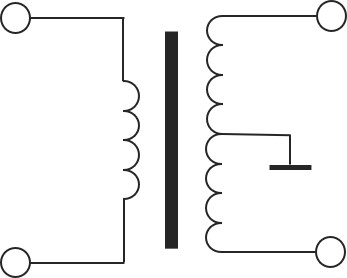
\includegraphics[width=0.3\linewidth]{Spannungsbalung.jpg}
	\caption{Einfaches Beispiel für einen Spannungsbalun}\label{fig:Spannungsbalun}
\end{figure}

\subsection{Strombalun}
\label{sec:strombalun}
Ein Strombalun zwingt der Leitung einen symmetrischen Strom auf. Dabei werden die störenden Mantelwellen idealerweise unterdrückt. Ein einfaches Beispiel für einen Strombalun ist in Abbildung \ref{fig:Strombalun} ersichtlich. Da sich bei dieser Schaltung die beiden Magnetfelder für das gewünschte Gegentaktsignal aufheben, fliesst nur die Energie des störenden Signals als Magnetfeld durch den Kern. Dieser darf deshalb eine niedrigere Güte haben. Das kann sogar gewünscht sein, da dadurch das störenden Gleichtaktsignal in Wärme umgewandelt wird und eine tiefe Güte ausserdem einen breitbandigen Betrieb ermöglicht. Aufgrund der Eigenschaft dass der Strombalun Mantelwellen zumindest dämpft, kann er auch bei nicht idealen Dipolantennen verwendet werden. Eine Impedanzanpassung ist bei der klassischen Schaltung in der Abbildung \ref{fig:Strombalun} nicht möglich.
\begin{figure}[H]
	\centering
	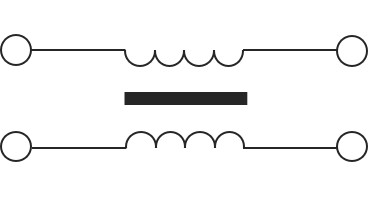
\includegraphics[width=0.3\linewidth]{Strombalun.jpg}
	\caption{Einfaches Beispiel für einen Strombalun}\label{fig:Strombalun}
\end{figure}

\newpage
\subsubsection{Guanella-Balun}
Der Guanella-Balun ist ein Spezialfall des Strombaluns, bei welchem durch Zusammenschalten von mehreren klassischen Stufen eine Impedanzanpassung für bestimmte Verhältnisse erreicht werden kann. In Abbildung \ref{fig:Guanella} ist ein Beispiel mit zwei Stufen ersichtlich. Unter der Annahme, dass die beiden Strombalune ideal funktionieren, fliessen die mit orangen Pfeilen eingezeichnete Ströme. Auf der linken Seite addieren sich je zwei Strompfade zusammen, wodurch der Strom, welcher von links in den Balun fliesst, doppelt so gross ist, wie der Strom auf der auf rechten Seite. Da die Schaltung idealerweise keine Verlustbehafteten Komponenten enthält muss die Eingangsleistung gleich gross wie die Ausgangsleistung sein. Daraus folgt, dass die Spannung auf der rechten Seite doppelt so gross wie links sein muss. Das Impedanzverhältniss berechnet sich wie folgt: \cite{balun_work} \cite{sevik} 
\begin{equation}
\frac{Z_2}{Z_1}=\frac{U_2/I_2}{U_1/I_1}=\frac{2\cdot U_1/I_2}{U_1/(2\cdot I_2)}=4:1
\label{equ:Guanella_1}
\end{equation}

Durch Hinzufügen von weiteren Stufen lassen sich folgende Verhältnisse realisieren:
\begin{equation}
	\frac{Z_{out}}{Z_{in}}=n^{2}:1 \hspace{1cm} n\in\mathrm{N}
\end{equation}
\begin{figure}[H]
	\centering
	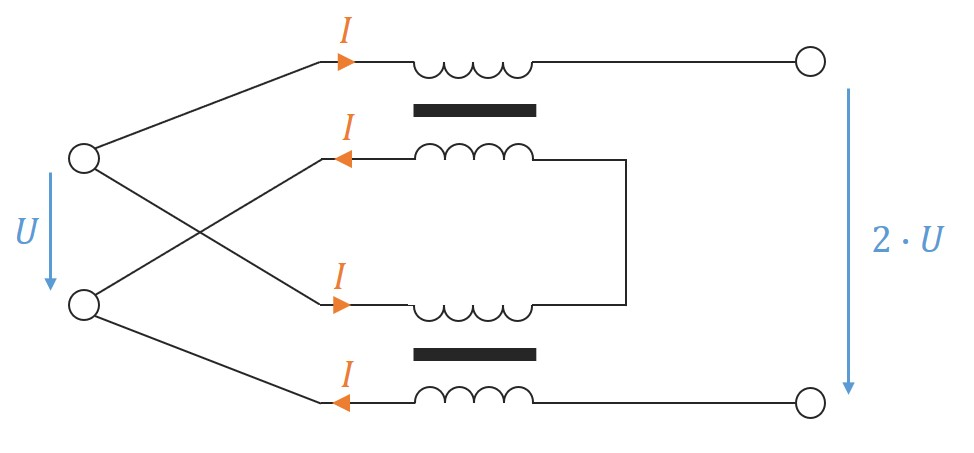
\includegraphics[width=1\linewidth]{Guanella.jpg}
	\caption{Ein Guanella-Balun mit zwei Stufen.}\label{fig:Guanella}
\end{figure}